\documentclass[12pt]{article}
\usepackage[utf8]{inputenc}
\usepackage[spanish]{babel}
\usepackage{geometry}
\usepackage[colorlinks=true, linkcolor=black, urlcolor=black, citecolor=black, pdfborder={0 0 0}]{hyperref}
\usepackage{listings}
\usepackage{xcolor}
\usepackage{graphicx}
\usepackage{subcaption}
\usepackage{caption}
\usepackage{float}

% Dirección de fotografias
\graphicspath{ {./fotos/} }

\geometry{letterpaper, margin=2.5cm}
\hypersetup{
    colorlinks=true,
    linkcolor=blue,
    urlcolor=blue,
    pdftitle={Instructivo de Instalación - Raspberry Pi},
    pdfauthor={Tu Nombre}
}

% Estilo para los comandos
\lstset{
  backgroundcolor=\color{lightgray!20},
  basicstyle=\ttfamily\small,
  frame=single,
  breaklines=true,
  postbreak=\mbox{\textcolor{red}{$\hookrightarrow$}\space},
  keywordstyle=\color{blue},
  commentstyle=\color{gray},
}
\begin{document}

\begin{titlepage}
    \centering
    \vspace*{2cm}

    {\Huge \textbf{Instructivo de Instalación del Sistema\\[0.5em] en Raspberry Pi} \par}
    \vspace{2cm}

    
\includegraphics[width=0.4\linewidth]{tiburoncin.jpg}
    \vspace{2cm}

    {\Large Ignacio Gutiérrez Arriagada \par}
    \vspace{0.5em}
    {\large \texttt{\href{mailto:gutierrezarriagada.ignacio@gmail.com}{gutierrezarriagada.ignacio@gmail.com}} \par}

    \vfill

    {\large \today\par}
\end{titlepage}


\section*{Resumen}

Este instructivo guía paso a paso el proceso de instalación y configuración básica de una Raspberry Pi para utilizarla en proyectos que requieren un entorno ligero, acceso remoto y ejecución automática de aplicaciones específicas. 

Comenzaremos con la instalación del sistema operativo Raspberry Pi OS Lite utilizando la herramienta oficial Raspberry Pi Imager. Se detallan todas las configuraciones necesarias, incluyendo la habilitación de conexión SSH y el acceso a red inalámbrica, para facilitar la administración remota del dispositivo.

Luego, se describe la instalación y configuración de un entorno gráfico mínimo basado en Openbox, pensado para ejecutar automáticamente la aplicación QGroundControl al iniciar el sistema, sin necesidad de entorno de escritorio completo.

A lo largo del documento se incluyen capturas de pantalla, comandos exactos y recomendaciones prácticas, todo explicado paso a paso, con énfasis en la comprensión por parte de usuarios no expertos, para que incluso quienes no estén familiarizados con estos procesos puedan seguirlo sin dificultades.

\newpage
\tableofcontents

\newpage
\section{Requisitos de Hardware y Software}
\subsection{Raspberry Pi 5}

Aunque el sistema ha sido desarrollado y optimizado para su ejecución en una \textbf{Raspberry Pi 5 con 8 GB de memoria RAM}, se ha verificado su correcto funcionamiento en una \textbf{Raspberry Pi 4 con 4 GB de memoria RAM}, garantizando así su compatibilidad con versiones anteriores desde ese modelo en adelante.

La \textbf{Raspberry Pi 5} presenta mejoras sustanciales en cuanto a arquitectura y rendimiento: incorpora una CPU ARM Cortex-A76 de cuatro núcleos a 2.4 GHz, mayor ancho de banda en memoria y buses, así como una GPU VideoCore VII con soporte mejorado para gráficos y procesamiento paralelo. Estas características permiten un manejo más eficiente de procesos intensivos en I/O, ejecución de aplicaciones gráficas como QGroundControl y operaciones de adquisición y procesamiento de datos en tiempo real.

Por otro lado, la \textbf{Raspberry Pi 4}, si bien posee una arquitectura basada en Cortex-A72 y una frecuencia de reloj menor, ofrece un entorno suficientemente estable y con recursos adecuados para ejecutar el sistema propuesto, siempre que cuente con al menos 4 GB de RAM. Esta condición asegura que no se produzcan cuellos de botella en la ejecución concurrente de servicios gráficos y tareas de comunicación o procesamiento.

Considerando los aspectos técnicos evaluados, el sistema puede ser implementado en cualquier Raspberry Pi desde la versión 4 (4 GB) en adelante, pero se recomienda utilizar la Raspberry Pi 5 para aprovechar al máximo el rendimiento del hardware y asegurar la escalabilidad de futuras actualizaciones o cargas de trabajo más exigentes.

\subsection{Raspberry Pi OS Lite}

Para la instalación de este sistema operativo se utilizó la herramienta ``\href{https://www.raspberrypi.com/software/}{Raspberry Pi Imager v1.8.5}'' para Windows, tal como se muestra en la Fig. \ref{RPI_IMAGER}.

\begin{figure}[H]
    \centering
    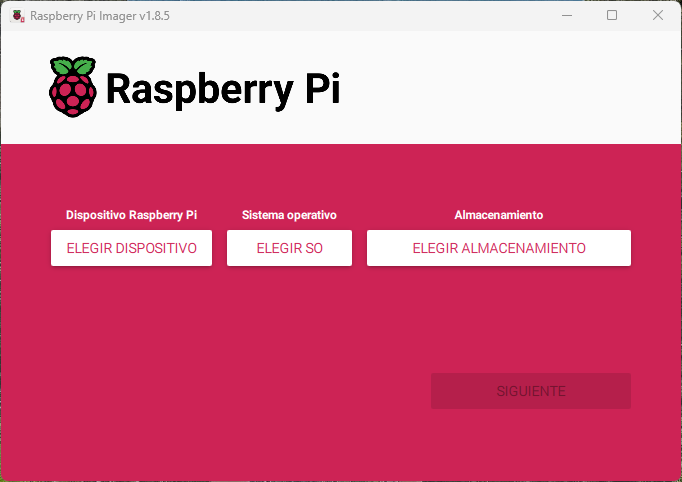
\includegraphics[width=10cm]{rpi_imager.png}
    \caption{Raspberry Pi Imager v1.8.5.}
    \label{RPI_IMAGER}
\end{figure}

Los parámetros a configurar en esta ventana del programa son los siguientes:

\begin{itemize}
    \item \textbf{Dispositivo Raspberry Pi:} seleccionar ``Raspberry Pi 5'' (o la placa que se esté utilizando).

        \begin{figure}[H]
            \centering
            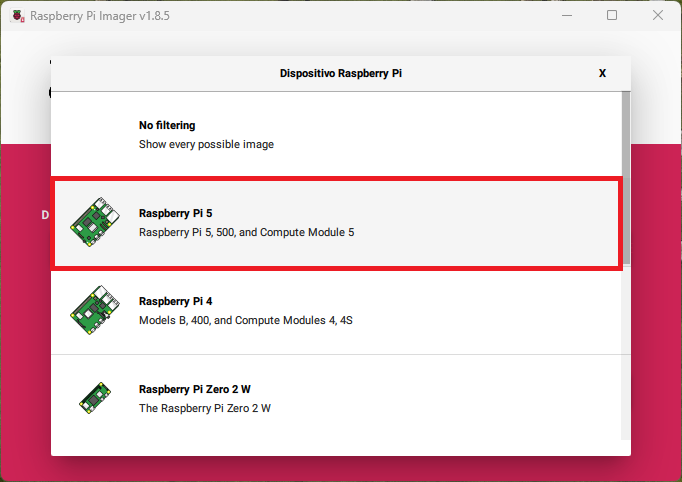
\includegraphics[width=10cm]{rpi_placa.png}
            \caption{Selección del modelo de placa.}
            \label{RPI_placa}
        \end{figure}

    \item \textbf{Sistema operativo:} seleccionar la opción ``Raspberry Pi OS (other)'' y luego ``Raspberry Pi OS Lite (64-bit)''.

        \begin{figure}[H]
            \centering
            \begin{subfigure}[b]{0.48\linewidth}
                \centering
                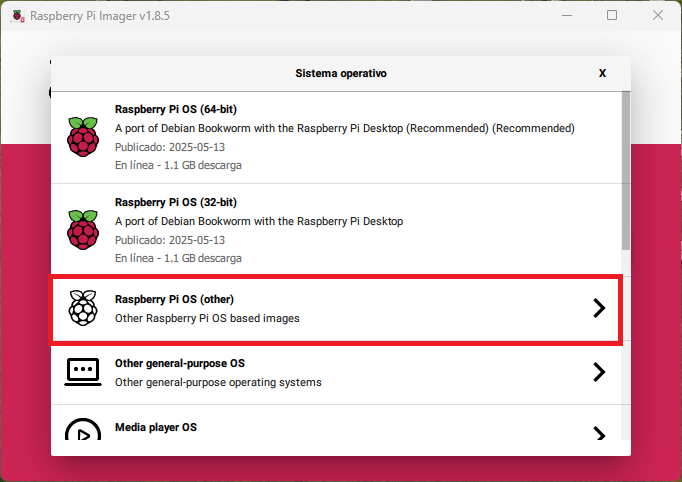
\includegraphics[width=\linewidth]{rpi_version1.png}
                \caption{Selección del tipo de sistema operativo.}
                \label{fig:rpi_version1}
            \end{subfigure}
            \hfill
            \begin{subfigure}[b]{0.48\linewidth}
                \centering
                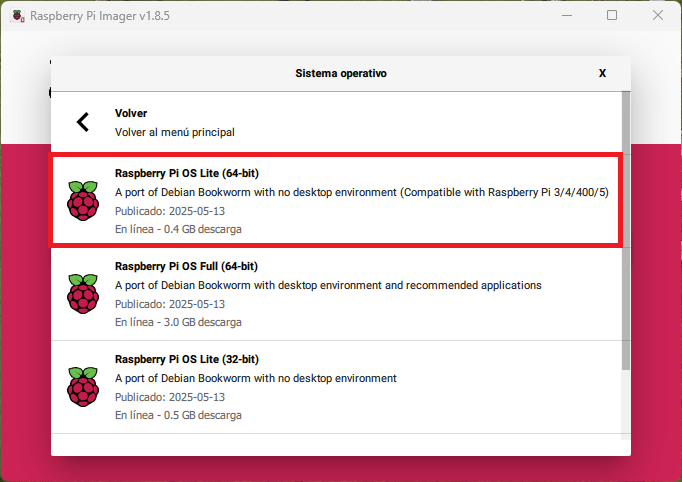
\includegraphics[width=\linewidth]{rpi_version2.png}
                \caption{Ubicación de Raspberry Pi OS Lite (64-bit).}
                \label{fig:rpi_version2}
            \end{subfigure}
            \caption{Elección del sistema operativo correcto.}
            \label{fig:rpi_versions}
        \end{figure}

    \item \textbf{Almacenamiento:} seleccionar la unidad de almacenamiento donde se instalará el SO.

        \begin{figure}[H]
            \centering
            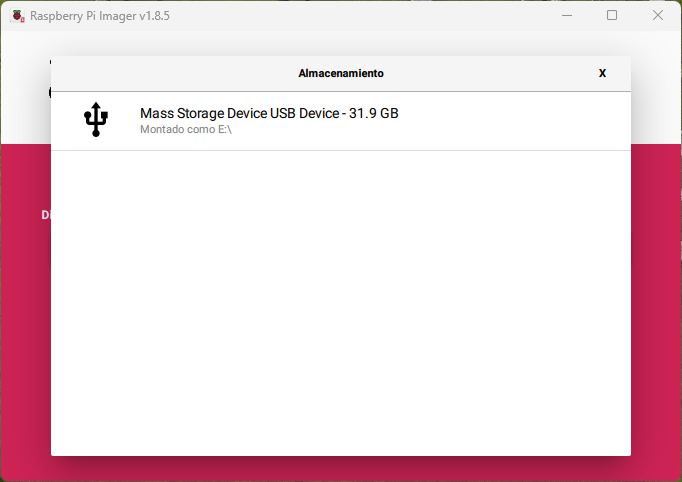
\includegraphics[width=10cm]{rpi_almacenamiento.png}
            \caption{Selección de la unidad de almacenamiento.}
            \label{RPI_ALMACENAMIENTO}
        \end{figure}
\end{itemize}

\subsection{Personalización del SO y habilitación de SSH}

Una vez configuradas todas las opciones en Raspberry Pi Imager, aparecerá una ventana emergente con el título ``¿Usar la personalización del SO?''. En esta ventana, se debe presionar la opción ``Editar ajustes'', como se muestra en la Fig. \ref{RPI_confirmacion}.

\begin{figure}[H]
    \centering
    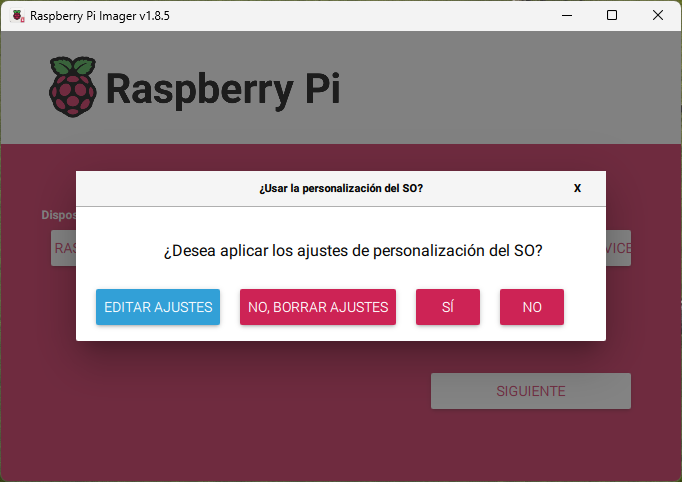
\includegraphics[width=10cm]{rpi_confirmacion.png}
    \caption{Confirmación para editar ajustes del sistema operativo.}
    \label{RPI_confirmacion}
\end{figure}

Al presionar este botón, se abrirá una nueva ventana llamada ``Personalización del SO'', donde se deben configurar los siguientes parámetros:

\begin{itemize}
    \item Nombre del anfitrión (hostname).
    \item Nombre de usuario.
    \item Contraseña de acceso al sistema.
    \item Conexión a red inalámbrica (SSID y Contraseña).
\end{itemize}

Todo esto se muestra en la Fig. \ref{fig:rpi_ajustes}. Para habilitar la conexión mediante \textit{SSH}, se debe presionar el botón ``Servicios'' y marcar las opciones correspondientes, como se muestra en la Fig. \ref{fig:rpi_ssh}.

\begin{figure}[H]
    \centering
    \begin{subfigure}[b]{0.48\linewidth}
        \centering
        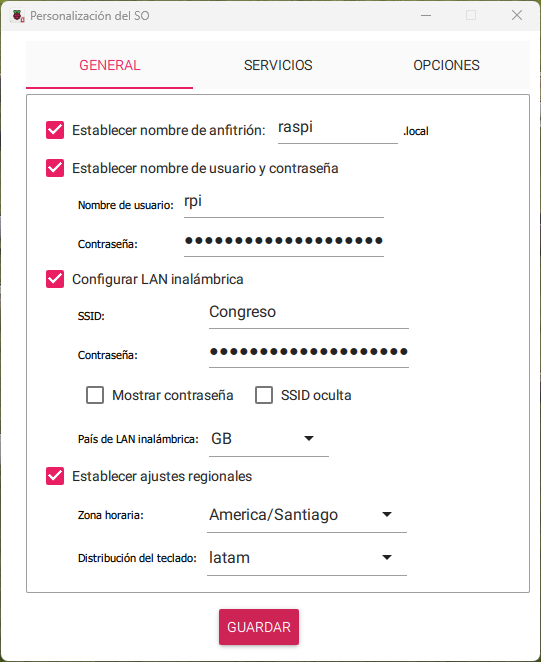
\includegraphics[width=\linewidth]{rpi_ajustes.png}
        \caption{Configuración general del sistema.}
        \label{fig:rpi_ajustes}
    \end{subfigure}
    \hfill
    \begin{subfigure}[b]{0.48\linewidth}
        \centering
        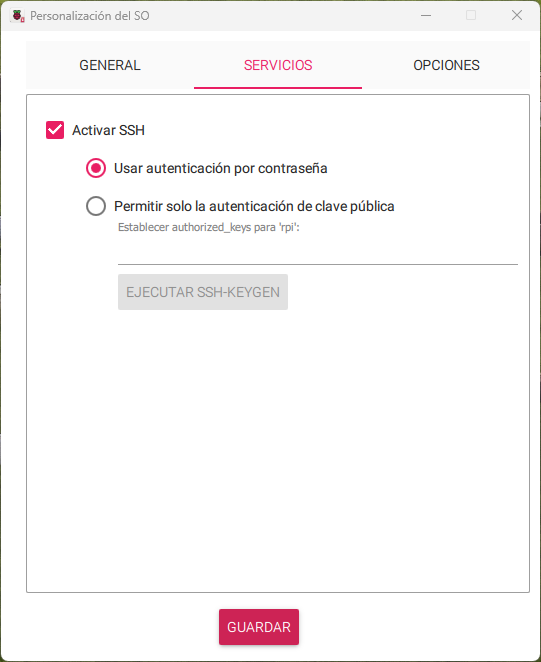
\includegraphics[width=\linewidth]{rpi_ssh.png}
        \caption{Habilitación del acceso SSH.}
        \label{fig:rpi_ssh}
    \end{subfigure}
    \caption{Ajustes personalizados del sistema operativo.}
    \label{fig:rpi_config}
\end{figure}

Una vez terminada la configuración y habilitado el acceso SSH, se debe presionar el botón ``GUARDAR''. Esto cerrará la ventana de personalización y volverá a mostrar la ventana emergente de Raspberry Pi Imager, donde ahora se debe presionar ``Sí'', como se ve en la Fig. \ref{fig:rpi_confirmacion1}.

Al hacer esto, se abrirá una nueva ventana con el título ``Advertencia'', donde se informa que todos los datos de la unidad seleccionada serán eliminados. Si se está seguro de continuar, presionar ``Sí'', como se aprecia en la Fig. \ref{fig:rpi_ultima_confirmacion}.

\begin{figure}[H]
    \centering
    \begin{subfigure}[b]{0.48\linewidth}
        \centering
        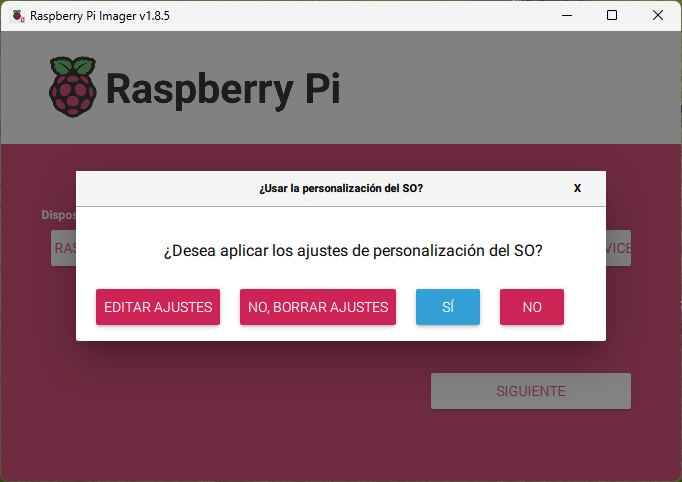
\includegraphics[width=\linewidth]{rpi_confirmacion1.png}
        \caption{Primera confirmación.}
        \label{fig:rpi_confirmacion1}
    \end{subfigure}
    \hfill
    \begin{subfigure}[b]{0.48\linewidth}
        \centering
        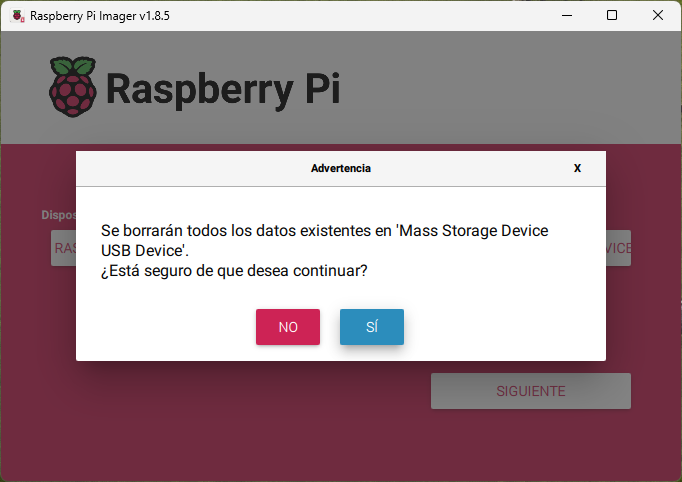
\includegraphics[width=\linewidth]{rpi_ultima_confirmacion.png}
        \caption{Confirmación final de escritura.}
        \label{fig:rpi_ultima_confirmacion}
    \end{subfigure}
    \caption{Proceso de confirmación durante la instalación.}
    \label{fig:rpi_confirmaciones}
\end{figure}

Luego de esto, se iniciará la descarga e instalación del sistema operativo en la tarjeta MicroSD. Una vez finalizada la escritura, se realizará una verificación automática. Se debe esperar hasta que aparezca la ventana emergente ``Escritura exitosa'', como se muestra en la Fig. \ref{RPI_listo}.

\begin{figure}[H]
    \centering
    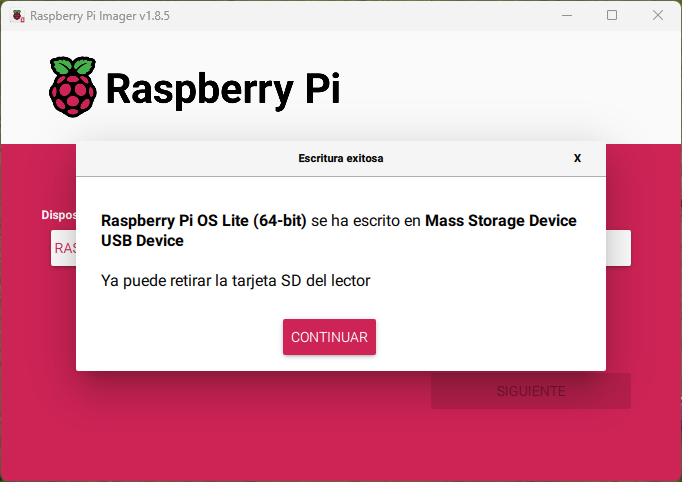
\includegraphics[width=10cm]{rpi_listo.png}
    \caption{Confirmación de instalación completada.}
    \label{RPI_listo}
\end{figure}

\newpage
\section{Configuración del entorno gráfico y herramientas}


\subsection{Acceso al SO mediante SSH}
Al iniciar por primera vez la Raspberry Pi con la tarjeta microSD insertada, se mostrará una consola simple con el siguiente encabezado:

\begin{itemize}
    \item \textbf{Debian GNU/Linux 12:} es la versión del sistema operativo instalado.
    \item \textbf{raspi:} corresponde al nombre del host definido durante la configuración del sistema operativo.
    \item \textbf{tty1:} representa el terminal virtual activo. ``tty'' significa ``teletypewriter'' y en este caso, indica que se está interactuando directamente con la consola física 1.
\end{itemize}

Debajo de esta línea, se mostrará la dirección IP asignada por la red (tanto IPv4 como IPv6), seguida por una línea de inicio de sesión que solicitará el nombre de usuario y la contraseña configurados previamente.

Es importante para conectarse mediante SSH, conocer la IP que le asignó la red a la placa, por lo que para este caso, se requiere verificar la segunda línea mencionada anteriormente, para así conectarse a través de un escritorio remoto mediante el siguiente comando:

\begin{lstlisting}
    ssh {rpi}@{IPv4}
\end{lstlisting}

En este caso específico, el nombre de usuario asignado fue \texttt{rpi} y la IPv4 asignada fue \texttt{172.17.36.2}, por lo que el comando a ingresar es:

\begin{lstlisting}
    ssh rpi@172.17.36.2
\end{lstlisting}

Una vez conectado a la placa mediante SSH, va a consultar si aceptas la ``\textit{fingerprints}'', a lo que se debe escribir \textit{yes}. Cabe mencionar que esto lo consultará sólo una vez. Una vez hecho esto, consultará por la contraseña del usuario con el cual se conectó mediante SSH, se ingresa y ya se tiene acceso total a la Raspberry Pi, con permisos de Super Usuario (conocido como \textit{sudo}).

\subsection{Actualización del sistema}

Antes de instalar cualquier herramienta, es recomendable actualizar el sistema operativo para asegurar compatibilidad y estabilidad.

\begin{lstlisting}
sudo apt update && sudo apt upgrade -y
sudo reboot
\end{lstlisting}

\subsection{Instalación de aplicaciones necesarias}

Se instalará Flatpak para permitir la descarga de aplicaciones desde Flathub. Luego se instala QGroundControl mediante este sistema.

\begin{lstlisting}
sudo apt install -y flatpak
sudo reboot
flatpak remote-add --if-not-exists flathub https://dl.flathub.org/repo/flathub.flatpakrepo
flatpak install flathub org.mavlink.qgroundcontrol
sudo reboot
\end{lstlisting}

Una vez instalado, debe verse como se demuestra en la Fig. \ref{flatpak}.

\begin{figure}[H]
    \centering
    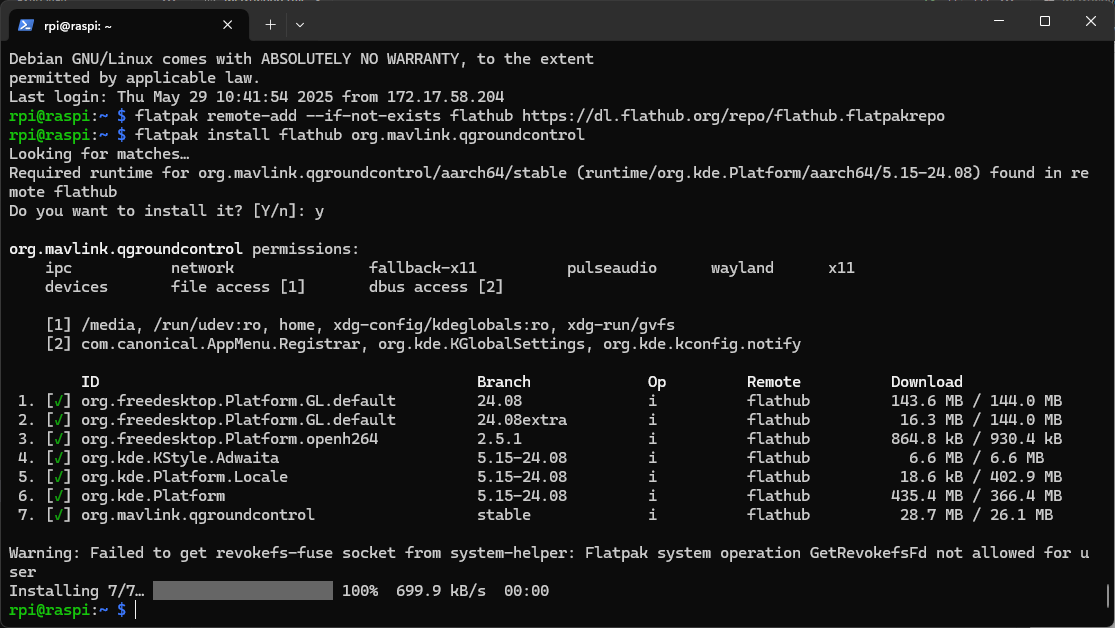
\includegraphics[width=10cm]{flatpak_installed.png}
    \caption{Flatpak instalado.}
    \label{flatpak}
\end{figure}

\subsection{Instalación del entorno gráfico mínimo}

Para ejecutar aplicaciones gráficas como QGroundControl, se instalará un entorno gráfico liviano basado en Openbox.

\begin{lstlisting}
sudo apt install -y xorg openbox unclutter xterm xdotool wmctrl libxcb-xinerama0 libxcb-icccm4 libxcb-image0 libxcb-keysyms1 libxcb-render-util0 libxcb-shape0 libxkbcommon-x11-0
\end{lstlisting}

\subsection{Configuración de Openbox}

Se configurará Openbox para que al iniciar el entorno gráfico se ejecute automáticamente QGroundControl.

\begin{lstlisting}
mkdir -p ~/.config/openbox
sudo nano ~/.config/openbox/autostart
\end{lstlisting}

\noindent
\textbf{Contenido de \texttt{autostart}:}

\begin{lstlisting}
#!/bin/bash

export DISPLAY=:0
xset -dpms
xset s off
unclutter &

sleep 3

flatpak run --env=QT_QPA_PLATFORM=xcb org.mavlink.qgroundcontrol &

sleep 5

WINDOW_ID=""
MAX_ATTEMPTS=10
ATTEMPTS=0
while [ -z "$WINDOW_ID" ] && [ $ATTEMPTS -lt $MAX_ATTEMPTS ]; do
    WINDOW_ID=$(xdotool search --name "QGroundControl")
    if [ -z "$WINDOW_ID" ]; then
        sleep 1
        ATTEMPTS=$((ATTEMPTS+1))
    fi
done

if [ -n "$WINDOW_ID" ]; then
    xdotool windowactivate "$WINDOW_ID" windowfullscreen "$WINDOW_ID"
fi
\end{lstlisting}

\begin{lstlisting}
sudo chmod +x ~/.config/openbox/autostart
\end{lstlisting}

\subsection{Configuración de inicio automático de sesión y entorno gráfico}

Esta configuración permite que el sistema inicie sesión automáticamente con el usuario \texttt{rpi} y ejecute el entorno gráfico sin intervención manual.

\begin{lstlisting}
    # Crear archivo .xinitrc
    sudo nano ~/.xinitrc     
\end{lstlisting}

Contenido de .xinitrc:

\begin{lstlisting}
exec openbox-session
\end{lstlisting}

\begin{lstlisting}
sudo mkdir -p /etc/systemd/system/getty@tty1.service.d
sudo nano /etc/systemd/system/getty@tty1.service.d/autologin.conf
\end{lstlisting}

Pegar esto:

\begin{lstlisting}
[Service]
ExecStart=
ExecStart=-/sbin/agetty --autologin rpi --noclear %I $TERM
\end{lstlisting}

\noindent
Luego se crea el archivo \texttt{.bash\_profile} para lanzar el entorno gráfico automáticamente:

\begin{lstlisting}
sudo nano ~/.bash_profile
\end{lstlisting}

\noindent
Contenido del archivo:

\begin{lstlisting}
if [[ -z $DISPLAY ]] && [[ $(tty) = /dev/tty1 ]]; then
    exec startx
fi
\end{lstlisting}

Finalmente:

\begin{lstlisting}
sudo systemctl daemon-reload
sudo reboot
\end{lstlisting}

\subsection{Verificación del funcionamiento}
Si todo fue configurado correctamente, al encender la Raspberry Pi debería verse directamente la interfaz de QGroundControl en pantalla completa. Si no es así, verificar lo siguiente:

\begin{itemize}
    \item La variable \texttt{DISPLAY} esté correctamente exportada.
    \item Que los permisos de ejecución estén otorgados al archivo \texttt{autostart}.
    \item Que la instalación de Flatpak y QGroundControl se haya completado sin errores.
\end{itemize}
\end{document}